\scanpage{50}%
\mspage{\handwritten{18}}%
rien, il s'ensuit que l'un des $K_i$ est déjà réduit au groupe unité, donc que $G\handwritten{\to}\underline{\operatorname{Aut}}_{\inserted{\handwritten{V_i}}}\deleted{\unsure{(V_i)}}$ est un monomorphisme. C'est donc une immersion fermée en vertu de (1.4.2), ce qui prouve que (iv)$\handwritten{\Rightarrow}$(v). Comme (\deleted{\unsure{g|8}}v)$\handwritten{\Rightarrow}$(i) triviale-\linebreak ment, cela prouve 11.11\deleted{\unsure{.|,}} pour $G$ de type fini.

\deleted{Prenons maintenant le cas général, où il reste à prouver que (iv)$\handwritten{\Rightarrow}$(i). Avec les notations de la démonstration précédente, soit $G_i$ le\inserted{plus petit} sous-groupe fermé de $\operatorname{Aut}(V_i)$ par le\deleted{q}\handwritten{q}\unsure{\deleted{eu}\handwritten{ue}|\deleted{ue}\handwritten{eu}}l\inserted{peut} se factoriser $G\handwritten{\to}\underline{\operatorname{Aut}}_{\inserted{\handwritten{V_i}}}\deleted{(V_i)}$ \deleted{(existe} (un tel groupe existe, \deleted{puisque} comme intersection de tous ceux par lesquels se factorise $G\handwritten{\to}\deleted{\unsure{\operatorname{Aut}(V_i)|\operatorname{Aut}(V_j)}}\inserted{\underline{\operatorname{Aut}}_{V_i}}$). Si $V_j\handwritten{\supset}V_i$, on voit alors tout de suite que $G_j$ invarie $V_i$ , et que le morphisme correspondant $G_j\handwritten{\to}\underline{\operatorname{Aut}}_{V_i}$ se facto-\linebreak rise par $G_i$ . De cette façon, les $G_i$ forment un système projectif de grou-\linebreak pes affines sur $k$, et on a un morphisme naturel $G\handwritten{\longrightarrow}G'=\underset{\handwritten{\longleftarrow}}{\lim}G_i$ , où $G'$ e\deleted{\unsure{z|s}}st lui-même un groupe affine (EGA IV 8.2.3). L'hypothèse que $G$ opère \uline{fidèlement} sur $V$ s'exprime alors par\deleted{l} le fait que $G\handwritten{\to}G'$ est un monomor-\linebreak phisme. On a donc trouvé\handwritten{/}un monomorphisme de $G$ dans un schéma affine, ce qui implique que le schéma quasi-comp\deleted{\unsure{c|e}}\handwritten{a}\deleted{t}\handwritten{c}t\inserted{et séparé} $G$ est quasi-affine, i.e. que son faisceau structural est ample, en vertu de EGA IV 18.12.17 . En \deleted{t}\handwritten{d}'autres termes, posant $H=\operatorname{Spec}\handwritten{\Gamma}(G,\underline{O}_G)$ , le morphisme canonique $G\handwritten{\to}H$ est une immersion ouverte. Notons maintenant que $H$ est de façon naturelle un schéma en groupes, et $G\handwritten{\to}H$ un homomorphisme de groupes, grâce à 11.2 . Cet homomorphisme est évidemment dominant, il reste à prouver que c'est un isomorphisme, ce qui résulte\deleted{ra d\unsure{e|a}} du lemme suivant:}
\margin{\handwritten{\handwritten{\makebox[0pt][l]{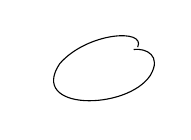
\begin{tikzpicture}[x=1cm,y=1cm,baseline=0pt]\draw (.39,.31).. controls (.5,.55) and (-.25,.5)..(-.6,.1).. controls (-1,-.5) and (.25,-.5)..(.55,-.05).. controls (.7,.2) and (.5,.3)..(.34,.28);\end{tikzpicture}}$\supset$}}}

\deleted{\uline{Lemme} 11.11.1.\handwritten{,} Soient $\deleted{\unsure{G|H}}\handwritten{H}$ un schéma en groupes sur un corps\inserted{$k$}\handwritten{.} \deleted{$\unsure{H|G}$ un sous-} Alors tout sous-schéma en groupes ouvert\inserted{$G$} de $H$ est aussi fermé.}
\margin{\handwritten{\figure{\begin{tikzpicture}\draw (0,0)--(.03,-.8);\end{tikzpicture}}}}

\deleted{Il revient au même de dire que l'ensemble $H-G$ est ouvert, i.e. est un voisinage de chacun de ses points\deleted{\unsure{,|;}} $x$ . Or , toute extension de corps $k'/k$ définissant un morphisme $\operatorname{Spec}k'\handwritten{\to}\operatorname{Spec}k$ qui est un\deleted{i}iversellement}
% archive sheet number: 49
